\documentclass[a4paper]{llncs}
\usepackage{amsmath}

\usepackage{tikz}
\usetikzlibrary{positioning}
\usetikzlibrary{calc}
\usetikzlibrary{arrows,shapes,backgrounds}

\newcommand{\vphi}{\vec{\varphi}}
\newcommand{\vi}{{\vec{i}}}
\newcommand{\vj}{{\vec{j}}}
\newcommand{\vmu}{\vec{\mu}}

\title{ GPU-accelerated and CPU SIMD Optimized \\ Monte Carlo Simulation of $\phi^4$ Model}
\author{Piotr Bialas \and Jakub Kowal \and Adam Strzelecki}
\institute{Faculty of Physics, Astronomy and Applied Computer Science\\
Jagiellonian University\\
ul. Reymonta 4, 30-059 Krakow, Poland }
\begin{document}


\maketitle



This contribution is concerned with an efficient implementation of the
Monte-Carlo simulations of the $\varphi^4$ model as defined in ref.~\cite{parisi}. The
problem is defined as follows: having a vector field $\vphi$ defined
on a regular rectangular two or three dimensional grid we want to
generate the field configurations with probability proportional to
\begin{equation}
e^{-H(\vphi)}
\end{equation}
where
\begin{equation}\label{eq:ham}\begin{split}
H(\varphi)&=\sum_{\vi}\Biggl(
\frac{1}{2}\sum_{\mu=1}^d(\vphi_{\vi+\hat{\mu}}-\vphi_{\vi})^2
+\frac{\mu^2}{2}|\vphi_{\vi}|^2+
\frac{g}{24}(|\vphi_{\vi}|^2)^2\\
&\phantom{=\sum_{\vi}\bigl(}+
\frac{1}{2\Lambda}\Bigl(\sum_{\mu=1}^d(\vphi_{\vi+\hat{\mu}}-2\vphi_{\vi}+\vphi_{\vi-\vmu})\Bigr)^2\Biggr).
\end{split}
\end{equation}
In the above expression $\vi$ denotes the grid point,
$\vphi_\vi$ denotes the $N$ component vector at the grid point $\vi$
 and $\vmu$ denotes the unit displacement on the grid in direction $\mu$.

The actual  generation is done by the mean of the Metropolis  algorithm as follows: for a given lattice point $\vj$ we produce a new field
\begin{equation}
\widetilde{\vphi}_\vj=\vphi_\vj+\vec{\epsilon}
\end{equation}
where $\epsilon$ is some random vector. The we calculate the difference
$\Delta H = H(\widetilde{\vphi})-H(\vphi)$.
We then replace $\vphi_\vj$ with $\widetilde{\vphi}_\vj$ with the probability
\begin{equation}
P=\max\left\{1,\exp(-\Delta H)\right\}.
\end{equation}
The crucial feature of this algorithm is that the $\Delta H$ depends
only on the immediate neighborhood of the point $\vj$. In our case
because of the last term in \eqref{eq:ham} this neighborhood is
extended compared to usual nearest neighbors (see figure~\ref{fig:nn} (Right)).
While model is inherently parallelizable, grid points
that lie in the same neighborhood cannot be updated together. That
proved to be a problem especially on the GPU where much more threads
access the grid in parallel.  Taking into account a larger
neighborhood means that a simple checkerboard decomposition pattern
cannot be used and we have devised a new grid decomposition
scheme.
\begin{figure}
\begin{center}
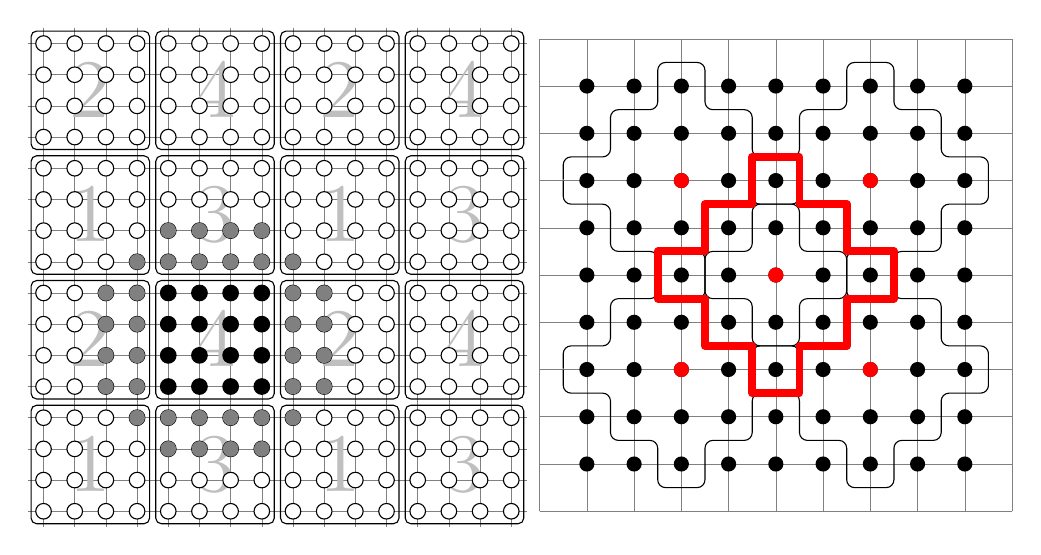
\begin{tikzpicture}[scale=0.6]
\begin{scope}[scale=0.66]
\draw[very thin, gray] (-0.5,-0.5) grid (15.5,15.5);

\foreach \x in {0,8}
\foreach \y in {0,8}
\draw[xshift=\x cm, yshift = \y cm]
node[lightgray,scale=3] at (1.5cm,1.5) {$1$}
node[lightgray,scale=3] at (1.5cm,5.5) {$2$}
node[lightgray,scale=3] at (5.5cm,1.5) {$3$}
node[lightgray,scale=3] at (5.5cm,5.5) {$4$} ;

\foreach \x in {0,...,15}
 \foreach \y in {0,...,15} {
  \fill[white] (\x, \y) circle(0.25);
  \draw[black] (\x, \y) circle(0.25);
}

\foreach \x in {4,...,7}
  \foreach \y in {4,...,7}
    \fill[black] (\x, \y) circle(0.25);

\foreach \x in {4,...,7}
  \foreach \y in {2,3,8,9}
    \fill[gray] (\x, \y) circle(0.25);

\foreach \x in {2,3,8,9}
  \foreach \y in {4,...,7}
    \fill[gray] (\x, \y) circle(0.25);

\foreach \p in {(3,3),(3,8),(8,3),(8,8)}
  \fill[gray] \p circle(0.25);

\foreach \x in {0,4,...,12}
  \foreach \y in {0,4,...,12}
    \draw[black,xshift=\x cm, yshift=\y cm, rounded corners = 2pt] (-.4,-0.4)
      rectangle (3.4cm,3.4cm);

\end{scope}

\begin{scope}[xshift=13.5cm,yshift=3cm]

\draw[help lines] (-3.0,-3.0) grid (7.0,7.0);

% lattice points
\foreach \x in {-2,-1,0,1,2,3,4,5,6}
  \foreach \y in {-2,-1,0,1,2,3,4,5,6}
    \fill (\x,\y) + (0.0,0.0) circle (0.16);

% neighborhood
\foreach \p in {(-2.5,4.0),(-2.5,-0.0),(1.5,4.0),(1.5,-0.0)}
  \draw[rounded corners=0.1cm,shorten >=2pt]
    \p-- ++(0,-0.5)-- ++(1,0)-- ++(0,-0.5)-- ++(0,-0.5)-- ++(1,0)--
    ++(0,-1.0)-- ++(1,0)-- ++(0,1.0)-- ++(1,0)-- ++(0,1.0)-- ++(1,0)--
    ++(0,1)-- ++(-1,0)-- ++(0,1)-- ++(-1,0)-- ++(0,1)-- ++(-1,0)-- ++(0,-1)--
    ++(-1,0)-- ++(0,-1)-- ++(-1,0)-- ++(0,-0.6);

% main center neighborhood
\draw[line width=0.1cm,color=red,cap=round,join=round]
  (-0.5,2.0)-- ++(0,-0.5)-- ++(1,0)-- ++(0,-0.5)-- ++(0,-0.5)-- ++(1,0)--
  ++(0,-1.0)-- ++(1,0)-- ++(0,1.0)-- ++(1,0)-- ++(0,1.0)-- ++(1,0)--
  ++(0,1)-- ++(-1,0)-- ++(0,1)-- ++(-1,0)-- ++(0,1)-- ++(-1,0)-- ++(0,-1)--
  ++(-1,0)-- ++(0,-1)-- ++(-1,0)-- ++(0,-0.6);

\fill[red] (2,2) circle(0.16);
\fill[red] (0,4) circle(0.16);
\fill[red] (0,0) circle(0.16);
\fill[red] (4,0) circle(0.16);
\fill[red] (4,4) circle(0.16);

\end{scope}

\end{tikzpicture}
\end{center}
\caption{\label{fig:nn} (Left) The partition of the lattice into
  blocks. The blocks with same number are processed in parallel.
  (Right) Partitioning of the blocks into disjoint sublattices. Black
  points are proceses in parallel.}
\end{figure}


% GPU implementation
On GPU we adopt the hierarchical scheme from ref.~\cite{weigel}
suitably modified to account for bigger neighborhood.  We first divide
the whole lattice in blocks of $32\times 32$ points. Then we start a
kernel that process every forth block (see figure~\ref{fig:nn}).  Each
block is assigned to a block of 128 threads. Each thread is fetching
eight lattice points from global to shared memory (black points). Then
the border points lying outside the block are fetched by some of the
threads (gray points). The necessity to fetch those points greatly
increases the complexity of the code. After that each thread updates
one point from the first partition. Then after synchronization, next
partition is updated and so on. After processing all eight(2D) or 16
(3D) partitions the kernel writes the shared memory back into global
and new kernel is started processing next batch of blocks.  Two
``tricks'' are used to speed up the calculations. First we use so
called multi-hit Metropolis algorithm, where each lattice point is
updated several times (four to eight)) one after another. This is more
efficient as some of the precalculated values are already in
registers. Secondly we do the same on the level of blocks, updating
every block many times in a row (typically 25-50). Altogether in this
way we managed to achieve $0.13$ nanoseconds for single lattice field
update on \emph{NVIDIA GTX 470}, reaching around $430$ Gflops that is
$40\%$ of $1088$ Gflops peak performance of this device .


% CPU implementation
In order to provide unbiased CPU vs GPU speed up results we provide
multithreaded vectorized CPU implementation. It uses OpenMP for parallel
execution, CPU SSE/AVX and compiler vector extensions for vectorization.

What is unique to this implementation it does mimic GPU SIMT execution model.
So instead vectorizing only parts of the existing generic algorithm it does
process several field updates within single thread.



\begin{thebibliography}{9}
\bibitem{parisi} G.~Parisi ``Statistical Field Theory'' Chapter 5, Perseus Books Publishing (1998).
\bibitem{weigel} M.~Weigel, J. Comput. Phys. \textbf{231}, 3064 (2012).
\end{thebibliography}
\end{document}
